\documentclass{article}
\usepackage{graphicx} % Required for inserting images
\usepackage{tikz} 
\usetikzlibrary{graphs,graphs.standard}
\usepackage{amsmath}

\title{The Probabilistic Method}
\author{William Gvozdjak}
\date{November 2023}

\begin{document}

\maketitle

We have some combinatorial problem, and we want to prove that something exists. But there's a problem: it feels impossible to actually find that thing--we know that it's probably out there, but we have no idea how to actually find it. How can we prove that it exists? Enter: the probabilistic method.

Initially, it may seem counterintuitive to use probability in a purely combinatorial problem. But as we'll see, probability can quickly eliminate combinatorial problems that seem extremely difficult at first sight. Let's introduce how it works with an example.

Suppose we have a bunch of points, and then line segments between any pair of those points. For example, if we have four points, it'll look like this:

% \begin{center}
%     \begin{tikzpicture}
%         \graph { subgraph K_n [n=4,clockwise,radius=1.5cm] };
%     \end{tikzpicture} 
% \end{center}
\begin{center}
    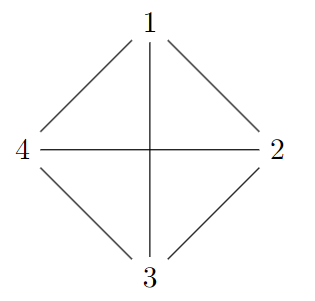
\includegraphics[width=4in]{images/K4.png}
\end{center}

This is called a \emph{complete graph} on $4$ vertices: each ``point'' is called a \emph{vertex}, and each line segment is called an \emph{edge}. We say that a \emph{complete subgraph} of this graph is any subset of its vertices together with all the edges between those vertices.

Let $k$ be some constant number. We're going to color each edge either red or blue. After this coloring, we want every single possible complete subgraph that has exactly $k$ vertices to have two edges that are different colors. In other words: is there some coloring such that every single complete subgraph with $k$ vertices has two edges that are different colors?

It seems completely strange that probability will be used in any way to solve this problem. But let's introduce probability! We color every edge in the graph randomly: for every edge, color it red with probability $\frac{1}{2}$ and blue with probability $\frac{1}{2}$. We're going to calculate the \emph{expected number} of subgraphs containing edges that are all the same color (if you don't know what expected value is, see the article from last month!).

To do this, let's consider one given subgraph, with $k$ vertices. Therefore, there are $\binom{k}{2}$ edges. We know that the probability that all its edges are one color is $2\cdot\left(\frac{1}{2}\right)^{\binom{k}{2}}=2^{1-\binom{k}{2}}$ (we need to multiply by $2$ since there are two possible colors, red and blue). The number of subgraphs that this will contribute to the total expected value is $1$, so this contributes $2^{1-\binom{k}{2}}$ to the total expected value. Otherwise, it'll contribute $0$, so the total expected value due to this subgraph is just $2^{1-\binom{k}{2}}$.

How many subgraphs are there in total? This is just $\binom{n}{k}$, where we have $n$ vertices in total. Therefore, the expected number of subgraphs that have all edges the same color is just
\[\binom{n}{k}\cdot 2^{1-\binom{k}{2}}.\]

Here's the cool part: let's say this number is less than $1$. Well, we know that the expected value is equal to the ``average'' value of whether a subgraph exists with all vertices the same color, if we randomly color all the vertices. This means that if the expected value is less than $1$, then there has to be some possible coloring that has value exactly equal to $0$--there has to be some coloring that has no subgraph with all edges the same coloring! As a result, we've provided one potential bound for $n$ and $k$: if
\[\binom{n}{k}\cdot 2^{1-\binom{k}{2}}<1\]
then there must exist some coloring of a complete graph with $n$ vertices such that every single complete subgraph with $k$ vertices has two edges that are different colors.

With this problem, we've seen how powerful the probabilistic method is: we didn't need to drudge through any difficult constructions of such a graph--it just magically popped out. Indeed, the probabilistic method is much, much deeper than just this problem, and has been repeatedly used to reduce complex problems into simple probability problems.

\end{document}
